\begin{answer}
Regularized loss curves

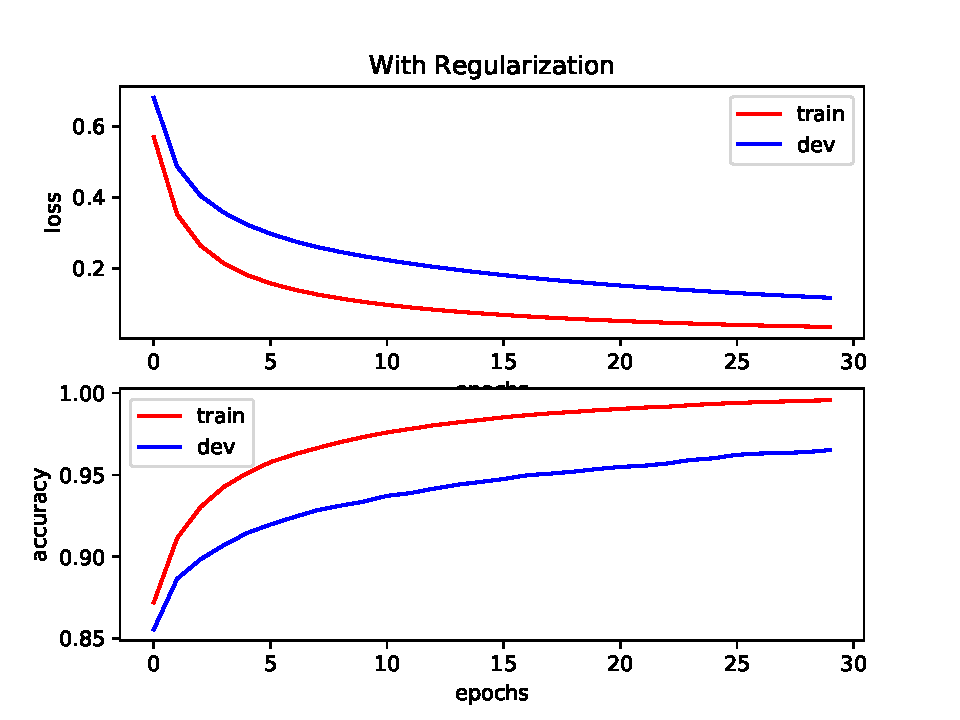
\includegraphics[scale=0.75]{../src/mnist/regularized}

The gap of accuracy between training set and dev set is smaller for regularize version.
Regularization helps avoid over-fitting!\\

\textbf{Note: \\ Derivation of the gradients for mini-batch gradient descent with regularization:}
The gradients of $J_{MB}$ with respect to the weight terms with the regularization term change to:

\begin{align*}
\nabla_{W^{[2]}} J_{MB} &=
\frac{1}{B} a^T  \cdot \left( \hat{y} - y \right) + 2 \lambda W^{[2]} & &\in \mathbb{R}^{h \times K}\\
\nabla_{W^{[1]}} J_{MB} &=
\frac{1}{B} X^T \left[ a \odot (1-a) \odot
\left( \hat{y} - y \right) \cdot W^{[2]T} \right]  + 2 \lambda W^{[1]} & &\in \mathbb{R}^{d \times h}
\end{align*}

The gradients with respect to the bias/intercept terms are not affected by regularization.
  
\end{answer}
   
  
